\newcommand*{\xMin}{0}%
\newcommand*{\xMax}{12}%
\newcommand*{\yMin}{0}%
\newcommand*{\yMax}{1}%
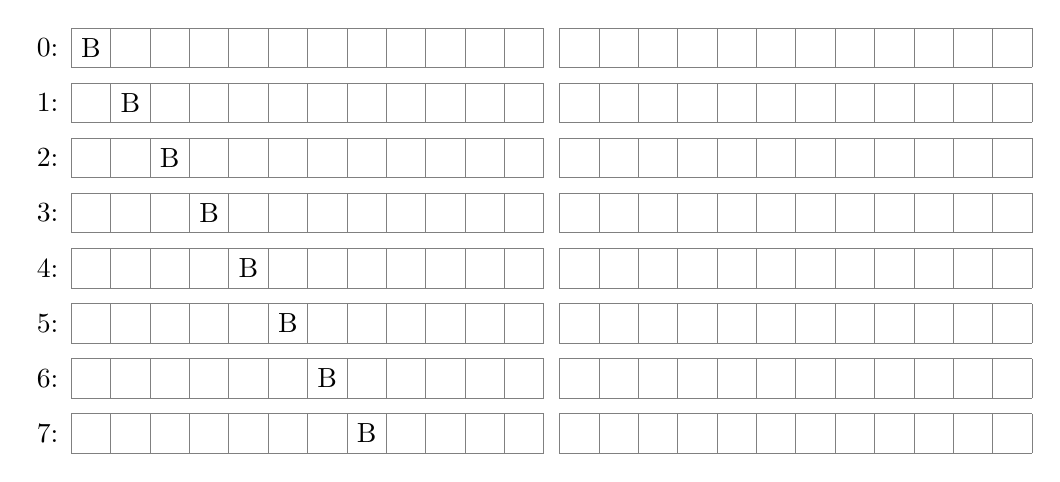
\begin{tikzpicture}
%   \foreach \i in {\xMin,...,\xMax} {
%       \draw [very thin,gray] (\i,\yMin) -- (\i,\yMax)  ;
%   }
%   \foreach \i in {\yMin,...,\yMax} {
%       \draw [very thin,gray] (\xMin,\i) -- (\xMax,\i) ;
%   }
    \foreach \j in {0,0.7,1.4,2.1,2.8,3.5,4.2,4.9} {
    \foreach \i in {0,0.5,1.0,1.5,2.0,2.5,3.0,3.5,4.0,4.5,5.0,5.5,6.0} {
        \draw [very thin,gray] (\i,\j) -- (\i,\j+0.5)  ;
        }

    \foreach \i in {\j,\j+0.5} {
        \draw [very thin,gray] (0,\i) -- (6.0,\i)  ;
        }


    \foreach \i in {0,0.5,1.0,1.5,2.0,2.5,3.0,3.5,4.0,4.5,5.0,5.5,6.0} {
        \draw [very thin,gray] (\i+6.2,\j) -- (\i+6.2,\j+0.5)  ;
        }

    \foreach \i in {\j,\j+0.5} {
        \draw [very thin,gray] (6.2,\i) -- (12.2,\i)  ;
        }
    }

    \node at (-0.3,0.25) {7: };
    \node at (-0.3,0.95) {6: };
    \node at (-0.3,1.65) {5: };
    \node at (-0.3,2.35) {4: };
    \node at (-0.3,3.05) {3: };
    \node at (-0.3,3.75) {2: };
    \node at (-0.3,4.45) {1: };
    \node at (-0.3,5.15) {0: };
    \node at (0.25,5.15) {B};
    \node at (0.75,4.45) {B};
    \node at (1.25,3.75) {B};
    \node at (1.75,3.05) {B};
    \node at (2.25,2.35) {B};
    \node at (2.75,1.65) {B};
    \node at (3.25,0.95) {B};
    \node at (3.75,0.25) {B};

  

\end{tikzpicture}
